\documentclass[hidelinks]{article}

%% Deutsche Silbentrennung und Sprache (neue Rechtschreibung)
\usepackage[ngerman]{babel}
%% Verwende Umlaute direkt
\usepackage[utf8x]{inputenc}
%% Hyperlinks für interne Referenzen
\usepackage{hyperref}
%% Grafiken einbinden
\usepackage{graphicx}
\usepackage{float}
%% Paket für Unterabbildungen pro Abbildung
\usepackage{subfig}


\usepackage{enumerate}
\usepackage{amsmath}
\usepackage{amssymb}

\usepackage{mathtools}
% Proof system
\usepackage{amsthm}

\theoremstyle{plain}
\newtheorem{thm}{Satz}[section]
\newtheorem{lem}[thm]{Lemma}

\theoremstyle{definition}
\newtheorem{defn}[thm]{Definition}
\newtheorem{bsp}[thm]{Beispiel}

\newtheoremstyle{rem} % name
    {\topsep}                    % Space above
    {\topsep}                    % Space below
    {}                   % Body font
    {}                           % Indent amount
    {\bf}                   % Theorem head font
    {:}                          % Punctuation after theorem head
    {.5em}                       % Space after theorem head
    {}  % Theorem head spec (can be left empty, meaning ‘normal’)

\theoremstyle{rem}
\newtheorem*{remark}{Bemerkung}

%\usepackage{xpatch}
%\makeatletter
%% Remove last point from definitions, theorems, etc.
%\xpatchcmd{\@thm}{\thm@headpunct{.}}{\thm@headpunct{\\}}{}{}
%\makeatother


% Seitenränder
\usepackage[margin=1.5in]{geometry}
% Zitate
\usepackage{cite}
% Tabellen
\usepackage[table]{xcolor}
\definecolor{lightblue}{HTML}{8ADAF2}
\definecolor{lightred}{HTML}{F2A28A}
\definecolor{lightgreen}{HTML}{A6F28A}
\definecolor{darkgreen}{HTML}{43A822}
\definecolor{grey}{HTML}{AAAAAA}


% Graphs
\usepackage{tikz}
\usepackage{tikz-3dplot}
\usepackage{pgfplots}
\usepgfplotslibrary{fillbetween}
\pgfplotsset{every axis/.append style={
                    axis x line=middle,    % put the x axis in the middle
                    axis y line=middle,    % put the y axis in the middle
                    axis line style={->,color=black}, % arrows on the axis
                    xlabel={$x$},          % default put x on x-axis
                    ylabel={$y$},          % default put y on y-axis
				}}

\setlength{\parindent}{0pt}

\newcommand{\pgtwo}{PG(2, $\mathbb{F}$)\ }
\newcommand{\fnz}{\mathbb{F}\setminus\{0\}}
\newcommand{\ftwnz}{\mathbb{F}^{2}\setminus\{\boldsymbol 0\}}
\newcommand{\ftnz}{\mathbb{F}^{3}\setminus\{\boldsymbol 0\}}
\newcommand{\pu}{\mathcal{P}_U}
\newcommand{\gu}{\mathcal{G}_U}

%Rename of Literatur to Literaturverzeichnis
\addto{\captionsngerman}{\renewcommand{\refname}{Literaturverzeichnis}}

% Titel der Arbeit
\title{Elliptische-Kurven-Kryptographie}
% Angaben zum Author
\author{Kevin Kappelmann, Lukas Stevens}
\pagestyle{plain}

%------------------------------------------------------------------------------
\begin{document}

\pagenumbering{gobble}
\maketitle
\vspace{6em}
\begin{figure}[H]
\centering
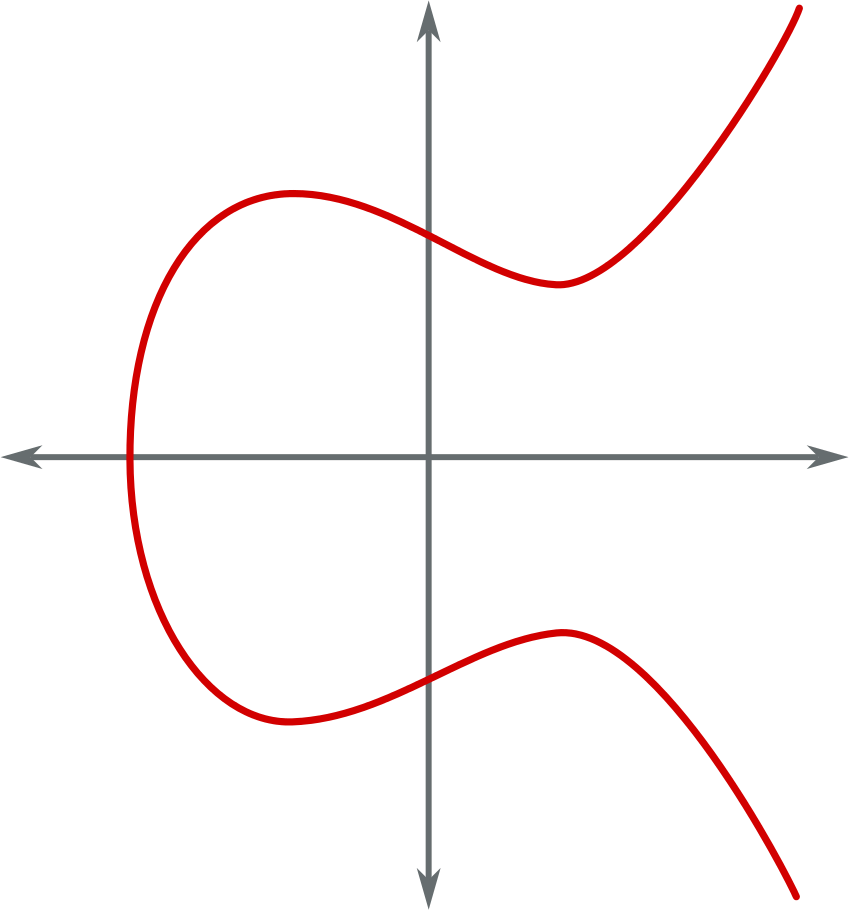
\includegraphics[scale=0.3]{cover}
\end{figure}

\newpage
\tableofcontents % Inhaltsverzeichnis
\listoffigures % Abbildungsverzeichnis
\listoftables % Tabellenverzeichnis 
\newpage

\pagenumbering{arabic}

\begin{sloppypar}

\section{Einleitung und Motivation}
Kryptosysteme wie RSA, Diffie-Hellman\footnote{In der jeweiligen Implementierung als Gruppe über ganze Zahlen} und ElGamal\footnotemark[\value{footnote}], die sich auf die Schwere der Primafaktorzerlegung bzw.\ dem diskreten Logarithmenproblem über Ganzzahlen stützen, benötigen sehr große Schlüssellängen, um eine ausreichend hohe Sicherheit zu garantieren. 
Daraus ergibt sich sowohl eine hoher Energie- als auch Speicherbedarf für die Berechnung der Algorithmen, was vor allem für Microchips und eingebettete Systeme ein Problem darstellt.\\
Eine Lösung für dieses Problem sind elliptische Kurven. Diese algebraischen Kurven tragen eine Gruppenstruktur, über die das diskrete Logarithmenproblem deutlich schwerer lösbar ist, als über Gruppen mit Ganzzahlen.
Kryptosysteme, die auf elliptische Kurven beruhen, kommen dadurch mit erheblich kürzeren Schlüsseln bei vergleichbarer Sicherheit aus.\cite[Seite~53]{nist}\\
Nachfolgende Tabelle verdeutlicht diesen Sachverhalt. Spalte 1 kennzeichnet die maximale Sicherheit (in Bits) für den jeweiligen Algorithmus und der angegebenen Schlüssellänge (in Bits). Rot markierte Felder gelten als kryptographisch unsicher, grüne als aktuell sicher.
\begin{table}[h]
\centering
	\begin{tabular}{| c | c | c |}
	\hline
	\rowcolor{lightblue}
	Sicherheitsniveau & RSA/Diffie-Hellman\footnotemark[\value{footnote}] & Elliptische-Kurven\\ \hline
	\rowcolor{lightred}
	$\le80$ 	& 1024 & 160-223 \\ \hline
	\rowcolor{lightgreen}
	112 	& 2048 & 224-255 \\ \hline
	\rowcolor{lightgreen}
	128 	& 3072 & 256-383 \\ \hline
	\rowcolor{lightgreen}
	192 	& 7680 & 384-511 \\ \hline
	\rowcolor{lightgreen}
	256 	& 15360 & 512+ \\ \hline
	\end{tabular}
\caption{Vergleich Schlüssellängen}
\end{table}

Die Verwendung elliptischer Kurven in der Kryptographie wurde Mitte der 1980er Jahre von Neal Koblitz\cite{koblitz} und Victor S. Miller\cite{miller} unabhängig voneinander vorgeschlagen. Aufgrund der vorteilhaften Eigenschaften gewinnt die \textbf{Elliptische-Kurven-Kryptographie} (kurz \textbf{ECC} für Elliptic Curves Cryptography) stets mehr an Bedeutung und löst ältere Verfahren wie RSA in den verschiedensten Bereichen ab. Vor allem in Umgebungen mit begrenzten Kapazitäten, wie z.B.\ Smartcards, ist ECC bereits weit verbreitet.\\
So verwendet beispielsweise Österreich seit 2004 als Vorreiter für alle gängigen Bürgerkarten ECC.\cite{austria} Aber auch die Reisepässe der meisten Europäischen Staaten nutzen inzwischen meist in einer Form ECC.\cite{eu}


\section{Grundbegriffe}
Um elliptische Kurven einführen zu können, müssen wir uns zunächst mit affiner und projektiver Geometrie und ihrer Verwandtheit auseinander setzen. Wir führen hierfür zunächst allgemein die Begriffe der affinen und projektiven Ebene ein und konstruieren uns eine projektive Ebene \pgtwo über einen beliebigen Körper $(\mathbb{F},+,*)$.\\\\
In den folgenden Kapiteln kürzen wir zu Gunsten der Notation den Körper $(\mathbb{F},+,*)$ mit $\mathbb{F}$ ab.\\


\subsection{Affine Ebenen}
\begin{defn}  \label{affine-ebene}
Es sei $\mathcal{A}$ eine Menge und $\mathcal{G}$ eine Teilmenge der Potenzmenge von $\mathcal{A}$, d.h. $\mathcal{G}\subseteq Pot(\mathcal{A})$.
Die Menge $\mathcal{A}$ nennt man die \textbf{Punktmenge} und die Menge $\mathcal{G}$ die \textbf{Geradenmenge} der affinen Ebene $(\mathcal{A},\mathcal{G})$, falls folgende drei Bedingungen erfüllt sind:
	\begin{enumerate}
		\item[(A1)] Zu je zwei Elementen $a, b\in \mathcal{A}$ mit $a\ne b$ existiert genau ein $G\in\mathcal{G}$ mit $a, b \in G$ (durch zwei verschiedene Punkte geht genau eine Gerade).\\
		Wir schreiben $\overline{a,b}$ für dieses G.
		\item[(A2)] Zu $G\in\mathcal{G}$ und $a\in\mathcal{A}\setminus G$ existiert genau ein $G'\in\mathcal{G}$ mit $a\in G'$ und $G\cap G'=\emptyset$ (durch jeden Punkt geht genau eine Gerade, die zu einer gegebenen Gerade parallel ist).\\
		Das sogenannte \textbf{Parallelenaxiom}.
		\item[(A3)] Es existieren drei Elemente $a,b,c\in\mathcal{A}$ mit $c\notin\overline{a,b}$ (es gibt drei Punkte, die nicht alle auf einer Gerade liegen).
	\end{enumerate}
\end{defn}

\begin{bsp}
Das \textbf{Minimalmodell} einer affinen Ebene umfasst genau 4 Punkte.\cite[Seite~16]{henn}
\begin{figure}[H]
\centering
\begin{tikzpicture}[scale=1.1,node distance=2.5cm,main node/.style={circle,fill=black,scale=0.75}]

\node at (0,0) [main node] (A) [label={[label]180:$a$}] {}; 
\node at (1.25,-2.5) [main node] (B) [label={[label]180:$b$}] {}; 
\node at (2.5,0)[main node] (D) [label={[label]0:$c$}] {};
\node at (1.25,-0.8) [main node] (C) [label={[label]0:$d$}] {};

\node at (3,-1.25) {$\boldsymbol\cong$};

\draw (A) -- (B) -- (C) -- (D) -- (A) -- (C)
      (D) -- (B);

\end{tikzpicture}
\begin{tikzpicture}[scale=1.1,node distance=2.5cm,main node/.style={circle,fill=black,scale=0.75}]

\node at (0,0) [main node] (A) [label={[label]180:$a$}] {}; 
\node at (0,-2.5) [main node] (B) [label={[label]180:$b$}] {}; 
\node at (2.5,-2.5)[main node] (C) [label={[label]0:$c$}] {};
\node at (2.5,0) [main node] (D) [label={[label]0:$d$}] {};

\draw (A) -- (B) -- (C) -- (D) -- (A) -- (C)
      (D) -- (B);
\end{tikzpicture}
\caption{Minimalmodell einer affinen Ebene}
\end{figure}

\end{bsp}

\begin{thm}
	Es sei $\mathbb{F}$ ein beliebiger Körper und $\mathbb{F}^2$ der zweidimensionale $\mathbb{F}$-Vektorraum mit Nullvektor $\boldsymbol 0$. Wir setzen
	\begin{equation*}
		\mathcal{G}\coloneqq\{a+\mathbb{F}b\mid a,b\in\mathbb{F}^2\land b\ne\boldsymbol 0\}
	\end{equation*}
	wobei $\mathbb{F}b=\{\lambda b\mid\lambda\in\mathbb{F}\}$ den von b erzeugten eindimensionalen Untervektorraum von $\mathbb{F}^2$ darstellt. Dann ist $(\mathbb{F}^2,\mathcal{G})$ eine affine Ebene.
\end{thm}
\begin{proof}
	Wir verweisen hier auf\cite[Seite~87]{karpfinger-kiechle}.
\end{proof}

\begin{bsp}
	Wählen wir für $\mathbb{F}$ den Körper $\mathbb{R}$, so erhalten wir für $(\mathbb{R}^2,\mathcal{G})$ die reelle affine Ebene (\textit{``Den zweidimensionalen Raum unserer Anschauung''}) mit Punkten und Geraden in der uns üblichen Interpretation.
\begin{figure}[H]
\centering
 \begin{tikzpicture}[scale=1,domain=-3:3] 
    \draw[step=1cm,very thin,color=gray] (-2.9,-2.9) grid (2.9,2.9);
    \draw[thick, ->] (-3.2,0) -- (3.2,0) node[right] {$x$}; 
    \draw[thick, ->] (0,-3.2) -- (0,3.2) node[above] {$y$};
    \foreach \x/\xtext in {-2, -1, 1, 2} 
	\draw (\x cm,1pt) -- (\x cm,-1pt) node[anchor=north,fill=white] {$\xtext$};
    \foreach \y/\ytext in {-2, -1, 1, 2} 
	\draw (1pt,\y cm) -- (-1pt,\y cm) node[anchor=east,fill=white] {$\ytext$};
    \draw[red] (-1.5,-0.5) node[right] {$a$};
    \draw[red] (1.5,2.5) node[right] {$b$};
    \draw[blue] (-1.5,-2.5) node[right] {$c$};
    \draw[blue] (1.5,0.5) node[right] {$d$};
    \draw[domain=-3:2,color=red]    plot (\x,1+\x)   node[right] {$\overline{a,b}$}; 
    \draw[domain=-2:3,color=blue]    plot (\x,-1+\x)   node[right] {$\overline{c,d}$};
    \filldraw[red] (-1.5,-0.5) circle[radius=2pt];
    \filldraw[red] (1.5,2.5) circle[radius=2pt];
    \filldraw[blue] (-1.5,-2.5) circle[radius=2pt];
    \filldraw[blue] (1.5,0.5) circle[radius=2pt];
    \draw (4,3) node[draw] {$\overline{a,b}\parallel\overline{c,d}$};
   \end{tikzpicture}
 \caption{Parallelen in der reellen affinen Ebene}
\end{figure}
\end{bsp}

\subsection{Projektive Ebenen}
\begin{defn} \label{projektive-ebene}
Es sei $\mathcal{P}$ eine Menge und $\mathcal{G}$ eine Teilmenge der Potenzmenge von $\mathcal{P}$, d.h. $\mathcal{G}\subseteq Pot(\mathcal{P})$.
Die Menge $\mathcal{P}$ nennt man die \textbf{Punktmenge} und die Menge $\mathcal{G}$ die \textbf{Geradenmenge} der projektiven Ebene $(\mathcal{P},\mathcal{G})$, falls folgende drei Bedingungen erfüllt sind:
	\begin{enumerate}
		\item[(P1)] Zu je zwei Elementen $P, Q\in \mathcal{P}$ mit $P\ne Q$ existiert genau ein $G\in\mathcal{G}$ mit $P, Q \in G$ (durch zwei verschiedene Punkte geht genau eine Gerade).\\
		Wir schreiben $\overline{P,Q}$ für dieses G.
		\item[(P2)] Für je zwei $G,H\in\mathcal{G}$ mit $G\ne H$ gilt $|G\cap H|=1$ (zwei verschiedene Geraden schneiden sich in genau einem Punkt).
		\item[(P3)] Es existieren vier verschiedene Elemente in $\mathcal{P}$, sodass immer höchstens zwei davon in jedem beliebigen $G\in\mathcal{G}$ liegen (es gibt vier Punkte, sodass nie drei davon auf derselben Gerade liegen).
	\end{enumerate}
\end{defn}
Im wesentlichen Unterschied zu affinen Ebenen existieren in einer projektiven Ebene \textbf{keine Parallelen}.

\begin{bsp}\label{fano}
Die \textbf{Fano-Ebene} ist das Minimalmodell einer projektiven Ebene und umfasst genau 7 Punkte (beachte: auch der Kreis gilt hier als Gerade!).\cite[Seite~9]{projmin}\\
Bemerkenswert ist die Tatsache, dass durch Entfernen einer beliebigen Gerade und den daraufliegenden Punkten eine affine Ebene entsteht. Dies ist kein Spezialfall sondern funktioniert immer, was wir auch im Abschnitt~\ref{konstr-aff-aus-proj} zeigen werden.
\begin{figure}[H]
\centering
\begin{tikzpicture}[node distance=1.5cm,main node/.style={circle,fill=black,scale=0.75}]

\node at (1.5,0) [main node] (A) [label={[label]180:$A$}] {}; 
\node at (0.63,-1.5) [main node] (B) [label={[label]180:$B$}] {}; 
\node at (-0.15,-3)[main node] (C) [label={[label]270:$C$}] {};
\node at (1.5,-3) [main node] (D) [label={[label]270:$D$}] {};
\node at (3.15,-3) [main node] (E) [label={[label]270:$E$}] {};
\node at (2.37,-1.5) [main node] (F) [label={[label]0:$F$}] {};
\node at (1.5,-2) [main node] (G) [label={[label]0:$G$}] {};

\draw (A) -- (B) -- (C) -- (D) -- (E) -- (F) -- (A)
	(B) -- (G) -- (D)
    (G) -- (F);
\draw (G) -- (E);
\draw (G) -- (A);
\draw (G) -- (C);

\draw (1.5,-2) circle [radius=1];

\end{tikzpicture}
\caption{Fano-Ebene}
\end{figure}
\end{bsp}


\subsubsection{Die projektive Ebene \pgtwo}
Es sei $\mathbb{F}$ ein beliebiger Körper mit Nullelement $0$ und $\mathbb{F}^3$ der dreidimensionale $\mathbb{F}$-Vektorraum mit Nullvektor $\boldsymbol 0$. Wir definieren eine Äquivalenzrelation~$\sim$ für alle $a,b\in\ftnz$ wie folgt:\\
\begin{equation*}
	a\sim b \Leftrightarrow \exists\lambda\in\fnz:\lambda a=b
\end{equation*}
Wir schreiben $[a]$ oder auch $(a_1:a_2:a_3)$ für die Äquivalenzklassen von $a=(a_1,a_2,a_3)\in\ftnz$.\\
Man bemerke: Für einen Vektor $a\in\ftnz$ stellt $[a]\cup\{\boldsymbol 0\}$ gerade den von a aufgespannten eindimensionalen Untervektorraum $\langle a \rangle=\mathbb{F}a=\{\lambda a\mid\lambda\in\mathbb{F}\}$ dar.\\

Weiters definieren wir uns die \textit{Quotientenmenge}, d.h.\ die Menge aller Äquivalenzklassen, als unsere Punktemenge:
\begin{equation*}
	\mathcal{P}\coloneqq(\ftnz)/\sim\ = \left \{[a]\mid a\in\ftnz\right \}
\end{equation*}
$\mathcal{P}$ stellt ein sogenanntes \textbf{homogenes Koordinatensystem} dar. Im Gegensatz zu den uns vertrauten (inhomogenen) Koordinaten, die jeden Punkt eindeutig identifizieren, haben homogene Koordinaten die Eigenschaft, dass sie für einen gegebenen Punkt nicht eindeutig bestimmt sind. So wird beispielsweise der Punkt $P=(2,4,8)\in\mathbb{R}^3$ sowohl von den homogenen Koordinaten $(1:2:4)$ als auch $(2:4:8)$ beschrieben.\\

Für zwei Punkte $P=[a],Q=[b]\in\mathcal{P}$ mit $P\ne Q$ setzen wir die Verbindungsgerade zwischen $P$ und $Q$ fest mit:
\begin{equation*}
	\overline{P,Q}\coloneqq\bigl \{[\lambda a+\mu b]\mid (0,0)\ne(\lambda,\mu)\in\mathbb{F}^2\bigr \}
\end{equation*}
Mit $\lambda=1$ und $\mu=0$ bzw.\ $\lambda=0$ und $\mu=1$ folgt direkt $P,Q\in\overline{P,Q}$.\\

Nun bilden wir noch die Menge aller Geraden:
\begin{equation*}
	\mathcal{G}\coloneqq\{\overline{P,Q}\mid P,Q\in\mathcal{P}\land P\ne Q\}
\end{equation*}
Man beachte, dass die Bedingung $[a]=P\ne Q=[b]$ gleichbedeutend ist mit der linearen Unabhängigkeit der Vektoren $a,b\in\mathbb{F}^3$. Für zwei Punkte $P,Q\in\mathcal{P}$ stellt $\overline{P,Q}\cup\{\boldsymbol 0\}$ also gerade den zweidimensionalen Untervektorraum $\langle a,b\rangle=\mathbb{F}a+\mathbb{F}b=\{\lambda a+\mu b\mid \lambda,\mu\in\mathbb{F}\}$ dar. 
Die Menge der Punkte einer Geraden $\overline{P,Q}$ entsprechen somit der Menge der eindimensionalen Untervektorräume, die jeweils als Teilmenge in $\mathbb{F}a+\mathbb{F}b$ enthalten sind. Formell ausgedückt:
\begin{equation*}
	[c]\in\overline{[a],[b]}\Leftrightarrow \mathbb{F}c\subseteq\mathbb{F}a+\mathbb{F}b\Leftrightarrow c\in\mathbb{F}a+\mathbb{F}b
\end{equation*}
\begin{defn}
	Es sei $V$ ein $n$-dimensionaler Vektorraum, $U$ ein beliebiger \mbox{$(n-1)$-dimensionaler} Untervektorraum von $V$ und $v\in V$ beliebig. Eine Teilmenge $H\subset V$ nennt man \textbf{Hyperebene} von $V$, wenn gilt:
\begin{equation*}
	H=v+U=\{v+u\mid u\in U\} 
\end{equation*}
\end{defn}
Wird für den Vektor $v$ der Nullvektor gewählt, so wird die erzeugte Ebene auch als \textit{lineare Hyperebene} bezeichnet.\\
In unserem Fall stellt also jede Gerade $\overline{P,Q}\cup\{\boldsymbol 0\}$ eine lineare Hyperebene über $\mathbb{F}^3$ dar.
\begin{thm}\label{hyperebene}
Es sei $V$ ein $n$-dimensionaler Vektorraum, $U$ ein beliebiger $(n-1)$-dimensionaler Untervektorraum von $V$ und $v\in V$ beliebig. 
Jede Hyperebene $H=v+U$ lässt sich für ein geeignetes $n\in V\setminus\{\boldsymbol 0\}$ äquivalent als Lösungsmenge einer homogenen linearen Gleichung beschreiben:
\begin{equation*}
	H=\{w\in V\mid \langle n,w-v\rangle=0\}
\end{equation*}
Wobei $\langle a,b\rangle$ das Standardskalarprodukt zweier Vektoren $a,b$ darstellt.
\end{thm}
\begin{proof}
	Wir verweisen hier auf\cite[Seite~189]{linalg}.
\end{proof}
\begin{remark}
Es ergibt sich, dass $n$ ein Normalenvektor zu $H$ sein muss.
\end{remark}
Satz~\ref{hyperebene} lässt eine alternative Definition unserer Geraden zu, die uns oft nützlich sein wird. Da alle Geraden $\overline{P,Q}\cup\{\boldsymbol 0\}$ lineare Hyperebenen sind, gilt nämlich für ein geeignetes \mbox{$n=(n_1,n_2,n_3)\in\ftnz$}:
\begin{equation*}
	\overline{P,Q}=\{(a_1:a_2:a_3)\in\mathcal{P}\mid n_1a_1+n_2a_2+n_3a_3=0\}
\end{equation*}
und somit
\begin{equation*}
	[c]\in\overline{P,Q}\Leftrightarrow n_1c_1+n_2c_2+n_3c_3=0
\end{equation*}

\begin{thm}
	Es ist \normalfont{\pgtwo}$\coloneqq(\mathcal{P},\mathcal{G})$ eine projektive Ebene über $\mathbb{F}$.
\end{thm}
\begin{proof}
	Wir müssen zeigen, dass die unter Definition~\ref{projektive-ebene} festgelegten Bedingungen (P1), (P2) und (P3) gelten.
\begin{enumerate}
	\item[(P1)] Es sei $P,Q\in\mathcal{P}$ mit $P\ne Q$. Durch Definition unserer Menge $\mathcal{G}$ folgt direkt $\overline{P,Q}\in\mathcal{G}$.\\
	Die Eindeutigkeit ergibt sich aus (P2).
	\item[(P2)] Es sei $G,H\in\mathcal{G}$ mit $P\ne Q$. Es gibt also zwei linear unabhängige Vektoren $(a,b,c),(a',b',c')\in\ftnz$ mit:
	\begin{align*}
	G & = \{(x:y:z)\in\mathcal{P}\mid ax+by+cz=0\}\quad\normalfont{und}\\
	H & =\{(x:y:z)\in\mathcal{P}\mid a'x+b'y+c'z=0\}
	\end{align*}
	Es folgt:
	\begin{equation*}
		G\cap H=\{(x:y:z)\in\mathcal{P}\mid ax+by+cz=0\land a'x+b'y+c'z=0\}
	\end{equation*}
	Dieses lineare Gleichungssystem hat als Lösungsmenge einen eindimensionalen Untervektorraum, also genau einen Punkt in $\mathcal{P}$. Folglich gilt $|G\cap H|=1$.
	\item[(P3)] Die vier Punkte $(1:0:0),(0:1:0),(0:0:1),(1:1:1)$ erfüllen die Bedingung.
\end{enumerate}
\end{proof}
\begin{bsp}
Mit Wahl von $\mathbb{F}=\mathbb{R}$ erhält man für PG(2,$\mathbb{R}$) die relle projektive Ebene, die über dasselbe Koordinatensystem, wie der euklidische Raum (\textit{``Der dreidimensionale Raum unserer Anschauung''}), definiert ist.\\
Die projektiven Punkte entsprechen den eindimensionalen Untervektorräumen von $\mathbb{R}^3$, d.h.\ die Menge aller Geraden durch den Ursprung und die Menge der projektiven Geraden entspricht analog der Menge aller Ebenen durch den Ursprung. Der Punkt $(0,0,0)$ ist dabei nicht enthalten.\\
Der Schnittpunkt zweier projektiven Geraden, d.h.\ anschaulich betrachtet zweier Ursprungsebenen, ergibt geanu eine Ursprungsgerade, also einen projektiven Punkt.\\
Wählt man zwei projektive Punkte $P,Q$, d.h.\ anschaulich betrachtet zwei Ursprungsgeraden, so ergibt sich als Verbindungsgerade $\overline{P,Q}$ die Ebene, die beide Geraden umfässt und durch den Ursprung verläuft.

\begin{figure}[H]
\tdplotsetmaincoords{80}{100}
\begin{tikzpicture}[
		tdplot_main_coords,
		axis/.style={->,black,thick},
		line/.style={thick,red},
		scale=0.8]

	% coordinates in (z,x,y)
	\filldraw[
		draw=darkgreen,%
		fill=darkgreen!20,%
	    ]          (-8,-2.5,0)
		    -- (-8,2.5,0)
		    -- (8,2.5,0)
		    -- (8,-2.5,0)
		    -- cycle;

	%draw the axes
	\draw[axis] (0,-3,0) -- (0,3,0) node[anchor=west]{$x$};
	\draw[axis] (0,0,-3) -- (0,0,3) node[anchor=west]{$y$};
	\draw[axis] (10,0,0) -- (-10,0,0) node[anchor=west]{$z$};

	\draw[line] (2,3,0) -- (-2,-3,0) node[anchor=east]{$P=[3:0:-2]$};
	\draw[line,blue] (6,3,0) -- (-6,-3,0) node[anchor=east]{$Q=[1:0:-2]$};
	\node[darkgreen] at (8,-3.0,0) {$\overline{P,Q}$};

\end{tikzpicture}
\qquad	
\tdplotsetmaincoords{80}{100}
\begin{tikzpicture}[
		tdplot_main_coords,
		axis/.style={->,black,thick},
		line/.style={thick,red},
		scale=0.8]

	% coordinates in (z,x,y)
	\filldraw[
		draw=darkgreen,%
		fill=darkgreen!20,%
	    ]          (0,-2.5,-2.5)
		    -- (0,-2.5,2.5)
		    -- (0,2.5,2.5)
		    -- (0,2.5,-2.5)
		    -- cycle;

	%draw the axes
	\draw[axis] (0,-3,0) -- (0,3,0) node[anchor=west]{$x$};
	\draw[axis] (0,0,-3) -- (0,0,3) node[anchor=west]{$y$};
	\draw[axis] (10,0,0) -- (-10,0,0) node[anchor=west]{$z$};

	\draw[line] (0,-3,-2) -- (0,3,2) node[anchor=west]{$P=[3:2:0]$};
	\draw[line,blue] (0,-3,-1) -- (0,3,1) node[anchor=west]{$Q=[3:1:0]$};
	\node[darkgreen] at (11,4.9,0) {$\overline{P,Q}$};

\end{tikzpicture}
	\caption{Punkte und Geraden projektiver reeller Ebenen}
\end{figure}
\end{bsp}


\subsubsection{Konstruktion affiner Ebenen aus projektiven Ebenen} \label{konstr-aff-aus-proj}
Wie wir bereits im Beispiel~\ref{fano} erkannt haben, erhält man durch Entfernen einer beliebigen Gerade einer projektiven Ebene und aller sich darauf befindenden Punkten, eine affine Ebene. Dies wollen wir nun beweisen.
\begin{thm} \label{projektive-zu-affinen}
Es sei $(\mathcal{P},\mathcal{G})$ eine projektive Ebene und $U\in\mathcal{G}$ beliebig. Wir definieren:
\begin{equation*}
	\pu\coloneqq\mathcal{P}\setminus{U},\quad \gu\coloneqq\left\{G\cap\pu\mid G\in\mathcal{G}\setminus\{U\}\right\}=\left\{G\setminus U\mid G\in\mathcal{G}\setminus \{U\}\right\}
\end{equation*}
Dann ist $(\pu,\gu)$ eine affine Ebene.
\end{thm}
\begin{proof}
Wir müssen zeigen, dass die unter Definition~\ref{affine-ebene} festgelegten Bedingungen (A1), (A2) und (A3) gelten.
\begin{enumerate}
	\item[(A1)] Zwei beliebige Punkte $P,Q\in\pu$ sind wegen (P1) durch genau eine Gerade verbunden. Diese Gerade wurde nicht entfernt, denn sonst wären auch auch die beiden Punkte $P,Q$ entfernt worden.
	\item[(A2)] Es sei $G_U\in\gu$, $G\in\mathcal{G}$ mit $G_U=G\setminus U$ und $P\in\pu\setminus G_U$. Die Gerade $G$ hatte wegen (P1) einen Schnittpunkt $F$ mit der Geraden $U$, der in $G_U$ entfernt wurde. Ebenfalls gibt es wegen (P1) eine Gerade $H_U\in\gu$ und eine Gerade $H\in\mathcal{G}$ mit $H_U=H\setminus U$, sodass $F,P\in H$. Da nach (P2) sich alle Geraden in genau einem Punkt schneiden und $H$ und $G$ sich im entfernten Schnittpunkt $F$ geschnitten haben, gilt $H_U\cap G_U=\emptyset$\\
	Jede andere Gerade in $\gu$ hat nach (P2) einen Schnittpunkt mit $G_U$, der nicht entfernt wurde. $H_U$ ist also die einzige Parallele von $G_U$ durch $P$.
\begin{figure}[H]
\centering
 \begin{tikzpicture}[scale=1,domain=0:4] 
    \draw[domain=0:4]    plot (\x,-0.5+1/2*\x)  node[right] {$H_U$}; 
    \draw[domain=0:4]    plot (\x,0)   node[right] {$G_U$};
    \draw[domain=0:4,red]    plot (\x,0.25-1/4*\x)   node[right] {$U$};
    \draw[red] (1,0) node[anchor=north] {$F$};
    \filldraw[red] (1,0) circle[radius=1.5pt];
    \draw (3,1) node[above] {$P$};
    \filldraw (3,1) circle[radius=1.5pt];
   \end{tikzpicture}
 \caption{Parallelen in \pgtwo nach Entfernen einer Geraden}
\end{figure}
	\item[(A3)] Wegen (P3) gibt es vier verschiedene Punkte $A,B,C,D\in\mathcal{P}$, sodass nie drei davon auf derselben Gerade liegen.\\
		Lag höchstens ein Punkt auf der entfernten Gerade $U$, folgt die Aussage mit den drei übrigen Punkten.\\
		Lagen zwei der vier Punkte auf $U$, o.B.d.A.\ sei dies $A,B$, so existiern zwei Geraden $\overline{A,C}$ und $\overline{B,D}$, die sich in einem Punkt $E$ schneiden, der nicht inzident zu $U=\overline{A,B}$ ist.
		Wäre nämlich $E$ inzident zu $\overline{A,B}$, dann würde aufgrund von (P1) $A\in\overline{B,D}$ und $B\in\overline{A,C}$ folgen, was im Widerspruch zur Annahme steht. Es gilt somit $E\in\pu$.\\
$E$ kann nicht inzident zu $\overline{C,D}$ sein, denn sonst würde aufgrund von (P1) $A,B\in\overline{C,D}$ gelten. Es folgt somit $E\notin\overline{C,D}$.
\begin{figure}[H]
\centering
 \begin{tikzpicture}[scale=1,domain=0:4] 
    \draw[red] (0,0) -- (4,0) node[right] {$U$};
    \draw (0.3,-0.3) -- (0.1,3);
    \draw (3.7,-0.3) -- (2,3);
    \draw (-0.5,2) -- (4,3);
    \draw (-0.34,2.46) -- (4,-0.3);
    \draw (0.07,-0.3) -- (2.87,3.5);

    \draw[red] (0.45,0) node[anchor=north] {$A$};
    \filldraw[red] (0.28,0) circle[radius=1.5pt];
    \draw[red] (3.38,0) node[below] {$B$};
    \filldraw[red] (3.55,0) circle[radius=1.5pt];
    \draw (2.1,2.7) node[left] {$C$};
    \filldraw (2.2,2.6) circle[radius=1.5pt];
    \draw (0.3,2.2) node[above] {$D$};
    \filldraw (0.16,2.15) circle[radius=1.5pt];
    \draw (1.32,1.38) node[below] {$E$};
    \filldraw (1.32,1.4) circle[radius=1.5pt];

   \end{tikzpicture}
 \caption{Nicht kollineare Punkte in \pgtwo nach Entfernen einer Geraden}
\end{figure}

\end{enumerate}
\end{proof}
\section{Elliptische Kurven $E$}
%Macht Lukas
\subsection{Die unendliche Gerade über \pgtwo}
%Isomorphismus von $\mathbb{F}^2 \rightarrow \mathcal{P}_U$
Um in~\ref{definition-ek} elliptische Kurven genau beschreiben zu können und in~\ref{affine-darstellung} eine affine Darstellung elliptischer Kurven herzuleiten, müssen wir $(\mathcal{P,G}) =$ \pgtwo nochmal betrachten.
Wir wählen dazu eine Gerade $U \in \mathcal{G}$ aus. 
Prinzipiell kann dazu jede Gerade gewählt werden. 
Es ist jedoch von Vorteil eine bestimmte Gerade zu wählen um das Rechnen mit der Weierstraßgleichung(\ref{weierstrass}) zu vereinfachen. \\
\newline
Dazu wählen wir die Verbindungsgerade $U = \overline{P,Q}$ der Punkte $P = (1:0:0)$ und $Q = (0:1:0)$, d.h.\ $U = \left\{ (x:y:z) \in \mathcal{P} \mid z = 0 \right\}$. 
Diese Menge $U$ bezeichnen wir im Folgenden als unendlich ferne Gerade.
Im dreidimensionalen Raum ist das genau die $x,y$-Ebene mit $z=0$. \\ 
\begin{lem}[Isomorphismus von $\pu$ und $\mathbb{F}^2$]
    Gegeben die projektive Ebene $(\mathcal{P}, \mathcal{G}) = PG(2,\mathbb{F})$ und die unendlich ferne Gerade $U$, dann ist die Abbildung
    \begin{equation*}
        \phi: \mathbb{F}^2 \rightarrow \mathcal{P}_U,\ (a,b) \mapsto (a:b:1)
    \end{equation*}
    bijektiv und bildet Geraden auf Geraden ab, d.h. $\phi$ ist ein Isomorphismus von affinen Ebenen. 
\end{lem}
\begin{proof} \label{isomorphismus-lemma}
    Wie im Satz~\ref{projektive-zu-affinen} gezeigt wurde, erhält man eine affine Ebene, wenn man aus einer projektiven Ebene eine Gerade mitsamt allen ihren Punkten entfernt. Daraus folgt, dass es sich bei $(\mathcal{P}_U, \mathcal{G}_U)$ um eine affine Ebene handelt. Es sei $(a:b:c) \in \mathcal{P}_U$. Da gilt $(a:b:c) \notin U$, folgt $c \neq 0$. Das heißt $c^{-1}$ ist definiert, womit die Abbildung
    \begin{equation*}
        \phi(ac^{-1},bc^{-1}) = (ac^{-1}:bc^{-1}:1) = (a:b:c)
    \end{equation*}
    surjektiv ist. Die Injektivität gilt auch, da mit $(a,b) \neq (a',b')$ die Vektoren $(a,b,1)$ und $(a',b',1)$ linear unabhängig sind, womit $(a:b:1) \neq (a':b':1)$ folgt. \\
    \newline
    Jede Gerade in $\mathbb{F}^2$ ist von der Form $\overline{a,b} = \left\{ a + \lambda b \mid \lambda \in \mathbb{F}\land a,b \in \mathbb{F}^2 \land b \neq \boldsymbol 0 \right\}$. Für einen Punkt $P = a + \lambda b \in \overline{a,b}$ gilt dann:
    \begin{equation*}
        \begin{aligned}
            \phi(a + \lambda b) & = (a_1 + \lambda b_1 : a_2 + \lambda b_2 : 1) = (a_1 : a_2 : 1) + \lambda (b_1 : b_2 : 0) \\
            & \sim \mu (a_1 : a_2 : 1) + \mu \lambda (b_1 : b_2 : 0)
        \end{aligned}
    \end{equation*}
    Hierbei ist zu beachten, dass $\mu \in \fnz$ laut Definition der Äquivalenzrelation $\sim$ gilt. Man betrachte nun die Gerade
    \begin{equation*}
        G \coloneqq \left\{ u(a_1 : a_2 : 1) + v(b_1 : b_2 : 0) \mid (u,v) \in \ftwnz\} \right\}.
    \end{equation*}
    Alle Punkte der Bildmenge von $\phi$ liegen auf der Gerade $G$. Es wird nur ein Punkt nicht erreicht, nämlich der Punkt $R = (b_1 : b_2 : 0)$. Wie man sehen kann, gilt $G \cap U = R$. Es folgt $\phi(\overline{a,b}) = G \cap \pu \in \gu$.
\end{proof}
Insgesamt kann man sehen, dass man affine Geraden auf eine Teilmenge der projektiven Geraden abbilden kann. Außerdem bekommen diese affinen Geraden im Projektiven dann einen Schnittpunkt, der auf der unendlich fernen Gerade $U$ liegt.
\subsection{Definiton elliptischer Kurven} \label{definition-ek}
%Weierstraßgleichung, Nullstellenmenge des Polynoms, Charakteristiken(Singularitäten), affine Koordinatentransformation?
Wir haben bereits die projektive Ebene \pgtwo über beliebige Körper $\mathbb{F}$ eingeführt.\\
Diese hat die folgende Punktemenge:
\begin{equation*}
    P = \left\{(u:v:w) \mid (u,v,w) \in \ftnz \right\}
\end{equation*}
Nun wollen wir die Punktemenge $E$ der elliptischen Kurve einführen, welche eine Teilmenge der Punktemenge $\mathcal{P}$ ist, d.h. $E \subseteq \mathcal{P}$. 
Dazu benötigen wir Polynome in drei Unbekannten.
Der Polynomring mit drei Unbekannten über $\mathbb{F}$ ist mit 
\begin{equation*}
    \mathbb{F}[X,Y,Z] = \left\{ \sum_{k,l,m \geq 0} a_{k,l,m} \thinspace X^k Y^l Z^m \mid a_{k,l,m} \in \mathbb{F} \right\}
\end{equation*}
definiert. 
$F(X,Y,Z) = \sum_{k,l,m \geq 0} a_{k,l,m} \thinspace X^k Y^l Z^m \in \mathbb{F}[X,Y,Z]$ wird Polynom genannt. 
\begin{defn}[Elliptische Kurve] \label{weierstrass}
    Eine elliptische Kurve $E$ ist durch die Lösung der Weierstraß-Gleichung 
    \begin{equation*}
        Y^2Z + a_1XYZ + a_3YZ^2 = X^3 + a_2X^2Z + a_4XZ^2 + a_6Z^3
    \end{equation*}
    gegeben, wobei $a_i \in \mathbb{F}$ gilt und die Lösung keine Singularitäten besitzen darf.\cite[Seite~54]{milne2006}
    Da der zugrundeliegende Raum \pgtwo eine projektive Ebene ist, handelt es sich um eine projektive Kurve. 
    Wenn man die Gleichung als Polynom 
    \begin{equation*}
        F(X,Y,Z) = Y^2Z + a_1XYZ + a_3YZ^2 - X^3 - a_2X^2Z - a_4XZ^2 -a_6Z^3
    \end{equation*}
    schreibt, dann ist $E$ genau die Nullstellenmenge des Polynoms $F$. Bemerkenswert ist hier, dass es sich um ein homogenes Polynom vom Grad 3 handelt, d.h.\ für jedes Summenglied $a_{k,l,m}X^kY^lZ^m$ mit $a_{k,l,m} \neq 0$ gilt $k + l + m = 3$.
\end{defn}
\begin{defn}[Singularitäten]
	Eine Kurve $E$ ist singulär in einem Punkt \mbox{$P=(a:b:c)\in E$}, wenn gilt
    \begin{equation*}
        \frac{\partial F}{\partial X}(P) = \frac{\partial F}{\partial Y}(P) =  \frac{\partial F}{\partial Z}(P) = 0
    \end{equation*}
    Man sagt auch, dass die partiellen Ableitungen des Polynoms $F$ im Punkt $P$ verschwinden. Falls die elliptische Kurve $E$ in keinem Punkt singulär ist, dann bezeichnet man sie als nicht-singulär.\cite[Seite~227]{karpfinger-kiechle}
\end{defn}
\begin{bsp}[Singularitäten]
    Die folgenden Kurven sind jeweils in einem Punkt singulär. Damit gibt es mehrere Tangenten an diesen Punkt.
    \begin{figure}[H]
        \centering
        \subfloat[$y^2=x^3+x^2$]{
            \begin{tikzpicture}
                \begin{axis}[
                    scale=0.8,
                    ticks = none,
                    axis equal,
                    restrict y to domain = -4:4,
                    restrict x to domain = -1:1.6,
                    ]
                    \addplot [color=red, domain = -4:4, samples = 300, unbounded coords=jump]
                    ({1/(x^3 - 1)}, { (x/(x^3 - 1))^1.5});
                    \addplot [color=red, domain = -4:4, samples = 300, unbounded coords=jump]
                    ({1/(x^3 - 1)}, {-(x/(x^3 - 1))^1.5}); 
                \end{axis}
            \end{tikzpicture}}
        \qquad
        \subfloat[$y^2=x^3$]{
            \begin{tikzpicture}
                \begin{axis}[
                    scale=0.8,
                    ticks = none,
                    axis equal,
                    ]
                    \addplot [color=red, domain=-2:2, samples=300, unbounded coords=jump]
                    {sqrt(x^3)};
                    \addplot [color=red, domain=-2:2, samples=300, unbounded coords=jump]
                    {-sqrt(x^3)};
                \end{axis}
            \end{tikzpicture}}
        \caption{Kurven mit Singularitäten (Knoten und Spitze)}
    \end{figure}
\end{bsp}
Wir hatten eine elliptische Kurve $E$ als Nullstellenmenge des Polynoms $F(X,Y,Z)$ mit \mbox{$E \coloneqq \left\{(u:v:w) \in \mathcal{P} \mid F(u,v,w) = 0 \right\}$} definiert.
Jedoch handelt es sich bei Punkten in der projektiven Ebene und damit auch bei den Elementen von $E$ um Äquivalenzklassen. Deswegen müssen wir noch die Wohldefiniertheit der Nullstellen begründen. 
Wir rufen uns dazu noch einmal die Definition der Äquivalenzrelation $\sim$ ins Gedächtnis: 
\begin{equation*}
	(u:v:w) \sim (u':v':w') \Leftrightarrow \exists \lambda \in \fnz: (u,v,w) = \lambda (u',v',w')
\end{equation*}
Wir setzen ein:
\begin{equation*}
    F(u',v',w') = F(\lambda u, \lambda v, \lambda w) = \lambda^3 F(u,v,w).
\end{equation*}
Die zweite Äquivalenz folgt aus der Homogenität des Polynoms. Daraus folgt, dass die Nullstellen von $F$ in $\mathcal{P}$ wohldefiniert sind:
\begin{equation*}
    F(u,v,w) = 0 \Leftrightarrow F(\lambda u, \lambda v, \lambda w) = 0.
\end{equation*}
Wir wollen nun noch eine Einschränkung treffen: die Charakteristik des Körpers $\mathbb{F}$ soll nicht 2 und nicht 3 sein. Wir schreiben $char \: \mathbb{F} \neq 2$ bzw.\ $char \: \mathbb{F} \neq 3$. 
Dies bedeutet, dass $1 + 1 \neq 0$ bzw.\ $1 + 1 + 1 \neq 0$, oder anders gesagt: Wenn wir das neutrale Element der Multiplikation 2 bzw.\ 3 mal addieren, dann erhalten wir nicht das neutrale Element der Addition, welches kein multiplikatives Inverses hat. 
Dadurch wird die Allgemeinheit für den Fall, dass $\mathbb{F}$ eine dieser Charakteristiken hat, eingeschränkt. \\
\newline
%Zitat? Seite 50 Milner
Wir können jetzt die Weierstraßgleichung(\ref{weierstrass}), welche die Form
\begin{equation*}
    Y^2Z + a_1XYZ + a_3YZ^2 = X^3 + a_2X^2Z + a_4XZ^2 + a_6Z^3
\end{equation*}
hat, umformen. Zuerst können wir, wenn $char \: \mathbb{F} \neq 2$ gilt, den Term $XYZ$ mit folgendem Variablenwechsel eliminieren:
\begin{equation*}
    X' = X, \: Y' = Y + \frac{a_1}{2} X, \: Z' = Z 
\end{equation*}
Anschließend könnnen wir auch noch die Terme $X^2$ und $Y$ eliminieren, falls $char \: \mathbb{F} \neq 2,3$ gilt:
\begin{equation*}
    X' = X + \frac{a_2}{3}, \: Y' = Y + \frac{a_3}{2}, \: Z' = Z
\end{equation*}
Damit lautet das Ergebnis
\begin{equation} \label{reduziert-weierstrass}
    Y^2Z = X^3 + aXZ^2 + bZ^3.
\end{equation}
\subsection{Affine Darstellung elliptischer Kurven} \label{affine-darstellung}
Wir wollen eine affine Darstellung herleiten. Dazu zeigen wir zunächst, dass nur ein Punkt der unendlich fernen Gerade $U$, nämlich der Punkt $\mathcal{O} = (0:1:0)$, auf $E$ liegt.
Für $P \in U$ gilt $P = (u:v:0)$ mit $u,v \in \mathbb{F}$. Es gibt drei Möglichkeiten Punkte zu erzeugen, die 0 als Z-Koordinate haben: $P = (1:0:0)$, $Q = (u:v:0)$ mit $u,v \in \fnz\}$ und $\mathcal{O} = (0:1:0)$. 
Wenn wir diese Punkte in die Gleichung~\ref{reduziert-weierstrass} einsetzen, dann löst nur $\mathcal{O}$ die Gleichung. \\ 
Für jeden Punkt $P \in E$ mit $P \neq \mathcal{O}$ gilt also $P \in \pu$. 
Aufgrund der Äquivalenzrelation $\sim$ können wir o.B.d.A.\ annehmen, dass $P \in \left\{(u:v:1) \mid u,v \in \mathbb{F} \right\}$. Wenn wir also nur diese Punkte betrachten, können wir die Gleichung~\ref{reduziert-weierstrass} vereinfachen und erhalten die affine Gleichung $y^2 = x^3 + ax + b$ oder als Polynom: 
\begin{equation} \label{affines-polynom}
    f(x,y) \coloneqq y^2 - x^3 - ax - b
\end{equation}
Wir wissen aus Satz~\ref{projektive-zu-affinen}, dass $\pu$ genau die Punktemenge einer affinen Ebene ist. Wenn wir zusätzlich die Abbildung $\phi$ aus Lemma~\ref{isomorphismus-lemma} auf $\pu$ anwenden, dann zerfällt die Punktemenge der elliptischen Kurve $E$ in zwei Teilmengen, einen affinen Teil und den unendlichen Punkt $\mathcal{O}$:
\begin{equation*}
    E = \left\{(u:v:1) \mid (u,v) \in \mathbb{F}^2 \land f(u,v) = 0 \right\} \cup \left\{ \mathcal{O} \right\}
\end{equation*}
Wir können im Anschluss nur den affinen Teil betrachten, wenn wir den Punkt $\mathcal{O}$ nicht außer Acht lassen.
\begin{bsp}
    Skizzen elliptischer Kurven über dem Körper $\mathbb{R}$
    \begin{figure}[H]
        \centering
        \subfloat[$y^2=x^3 + 0.3x + 2$]{
            \begin{tikzpicture}
                \begin{axis}[
                    no markers,
                    samples=800,
                    scale=0.8,
                    ]
                \addplot gnuplot{atanh(x)};
                \end{axis}
            \end{tikzpicture}}
        \qquad
        \subfloat[$y^2=x^3$]{
            \begin{tikzpicture}
                \begin{axis}[
                    scale=0.8,
                    axis equal,
                    ]
                    \addplot [color=red, domain=-2:2, samples=300, unbounded coords=jump]
                    {sqrt(x^3 - 2*x)};
                    \addplot [color=red, domain=-2:2, samples=300, unbounded coords=jump]
                    {-sqrt(x^3 - 2*x)};
                \end{axis}
            \end{tikzpicture}}
    \end{figure}
\end{bsp}
\section{Eine Gruppe über $E$}
Macht Kevin bis 4.3\\
\subsection{Tangenten elliptischer Kurven}
\subsection{Schnittpunkte von Geraden mit elliptischen Kurven}
Unendlich ferne Gerade mit Schnittpunkt $\mathcal{O}$, Affine Geraden, Parallele zur y-Achse
\subsection{Die Schnittpunkt-Verknüpfung $\oplus $ über $E$}
Definition, Beweis der Abgeschlossenheit, graphische Interpretation
\subsection{Die Gruppe $(E, +)$}
Macht Lukas bis fertig\\
Gruppe ist abelsch mit neutralem Element $\mathcal{O}$, Beispiel
\section{Anwendung elliptischer Kurven in der Kryptologie}
\subsection{ElGamal}
Welche Charakteristiken für elliptische Kurven, Domänenparameter
\subsection{Noch einen für Signaturen}
Welche Charakteristiken für elliptische Kurven, Domänenparameter

\end{sloppypar}
\newpage
\bibliographystyle{plain}
\bibliography{quellen}
\end{document}
